\documentclass[11pt]{article}

\usepackage{graphicx}
\usepackage{url}

\begin{document}

\begin{titlepage}
 \begin{center}
     
\includegraphics[scale=0.10]{du.png}\par
  \begin{Huge}
   \textsc{University of Dhaka}\par
  \end{Huge}
  \begin{Large}
   Department of Computer Science and Engineering\par \vspace{1cm}
   CSE-3111 : Computer Networking Lab \\[13pt] 
   Lab Report : Lab exercises on LAN configuration and troubleshooting tools 
  \end{Large}
 \end{center}   
 \begin{large}
  \textbf{Submitted By:\\[12pt]}
   Name : Md. Sadmin Tahmid Khan\\[8pt]
   Roll No : 35\\[12pt]
  \textbf{Submitted On : \\[12pt]}
    January 19, 2023\\[20pt]
  \textbf{Submitted To :\\[12pt]}
   Dr. Md. Abdur Razzaque\\[12pt]
                Md Mahmudur Rahman\\[12pt]
                Md. Ashraful Islam\\[12pt]
                Md. Fahim Arefin
 \end{large}
\end{titlepage}

\section{Introduction}
The preliminary objective of this lab is to know about LAN configuration and some troubleshooting tools. 
\subsection{Objectives}
\begin{itemize}
    \item To demonstrate a basic understanding of a LAN (Local Area Network) configuration.
    \item To demonstrate the ability of configuring and troubleshooting different types of LANs, such as Ethernet and Wi-Fi networks
    \item To demonstrate proficiency in using various troubleshooting tools, such as ping, traceroute, Ifconfig, nslookup etc.
    \end{itemize}
%%%%
%%%%
\section{Theory}
LAN (Local Area Network) configuration is the design and setup of a network that is used to connect devices within a small geographic area, such as in a house, office, or building. On the other hand, network troubleshooting tools are software or hardware tools that are used to diagnose and resolve issues with a network.
\section{Methodology}

\subsection{PING}
PING is a simple command-line tool that can be used to test connectivity between devices on a network.
\begin{itemize}
    \item \textbf{ping google.com:} testing internet connectivity of google
    \item \textbf{ping www.mit.edu:} testing internet connectivity of MIT's website, since it is located far from this location.
    \item \textbf{www.du.ac.bd} testing the internet connection of Dhaka University's site and caomparing it with MIT's.
\end{itemize}

\subsection{TRACEROUTE}
Traceroute is a command-line tool that can be used to trace the path of a packet of data from one device to another on a network.
\begin{itemize}
    \item \textbf{traceroute google.com:} to see the complete route of the google.com website
    \item \textbf{traceroute www.du.ac.bd:} to trace the path of Dhaka University's website.
    \item \textbf{traceroute www.mit.edu:} to trace the path of MIT's website and for comparing it with MIT's.
\end{itemize} 

\subsection{IFCONFIG}
Ifconfig (short for "interface configuration") is a command that can be used to display information about the current status of network interfaces, such as their IP addresses, netmasks, and other configuration settings.
\begin{itemize}
    \item \textbf{ifconfig:} It displays the current configuration for a network interface when no optional parameters are supplied
    \item \textbf{ifconfig -a:}: The ifconfig command with the -a argument will display information of all active or inactive network interfaces on the server. It displays the results for eth0, lo, sit0 and tun0
    \item \textbf{ifconfig eth0 up:} The “up” or “ifup” flag with interface name (eth0) activates a network interface if it is not inactive state and allowing to send and receive information.
    \item \textbf{ifconfig eth0 down:} The "dowm" flag with interface name(eth0) inactivates a network interface if it is not activate state.
    \end{itemize}
\subsection{ARP}
ARP (Address Resolution Protocol) is a protocol used to map a network layer protocol address (such as an IP address) to a link layer protocol address (such as a MAC address) on a local network. It is used to resolve IP addresses to physical (MAC) addresses on a LAN.
\begin{itemize}
    \item \textbf{arp -a:} show the IP addresses and corresponding MAC addresses of the devices that have recently communicated on the LAN.
\end{itemize}

\subsection{RARP}
RARP (Reverse Address Resolution Protocol) is a protocol that is similar to ARP, but it is used to map a link layer protocol address (such as a MAC address) to a network layer protocol address (such as an IP address). It is essentially the reverse of ARP, and it is used to resolve MAC addresses to IP addresses on a LAN.
\begin{itemize}
    \item \textbf{rarp -h:} view all commands relared to rarp
    \item \textbf{rarp -V:} Display program version
\end{itemize}

\subsection{NSLOOKUP}
nslookup (short for "name server lookup") is a command that is used to query DNS (Domain Name System) servers for information about a specific domain name or IP address. 
\begin{itemize}
    \item \textbf{nslookup google.com} this command is used to find the address record for a domain.
    \item \textbf{nslookup 10.33.2.78:} Reverse DNS lookup command.
    \item \textbf{nslookup -type=any google.com:} Lookup command for any record.
\end{itemize}

\subsection{NETSTAT}
Netstat (short for "network statistics") is a command that is used to display information about the current status of network connections on a system. It can be used to view information about active and listening TCP, UDP, and ICMP connections, as well as statistics on network traffic, such as the number of packets sent and received, and the number of errors.
\begin{itemize}
    \item \textbf{netstat -a:} it shows all active and listening connections, including TCP and UDP ports.
    \item \textbf{netstat -at:} it lists all tcp ports.
    \item \textbf{netstat -i:} it shows statistics about all the network interfaces.
\end{itemize}
\section{Experimental result}

Some Snapshots can be seen in the following figures: 
\begin{figure}
\centering
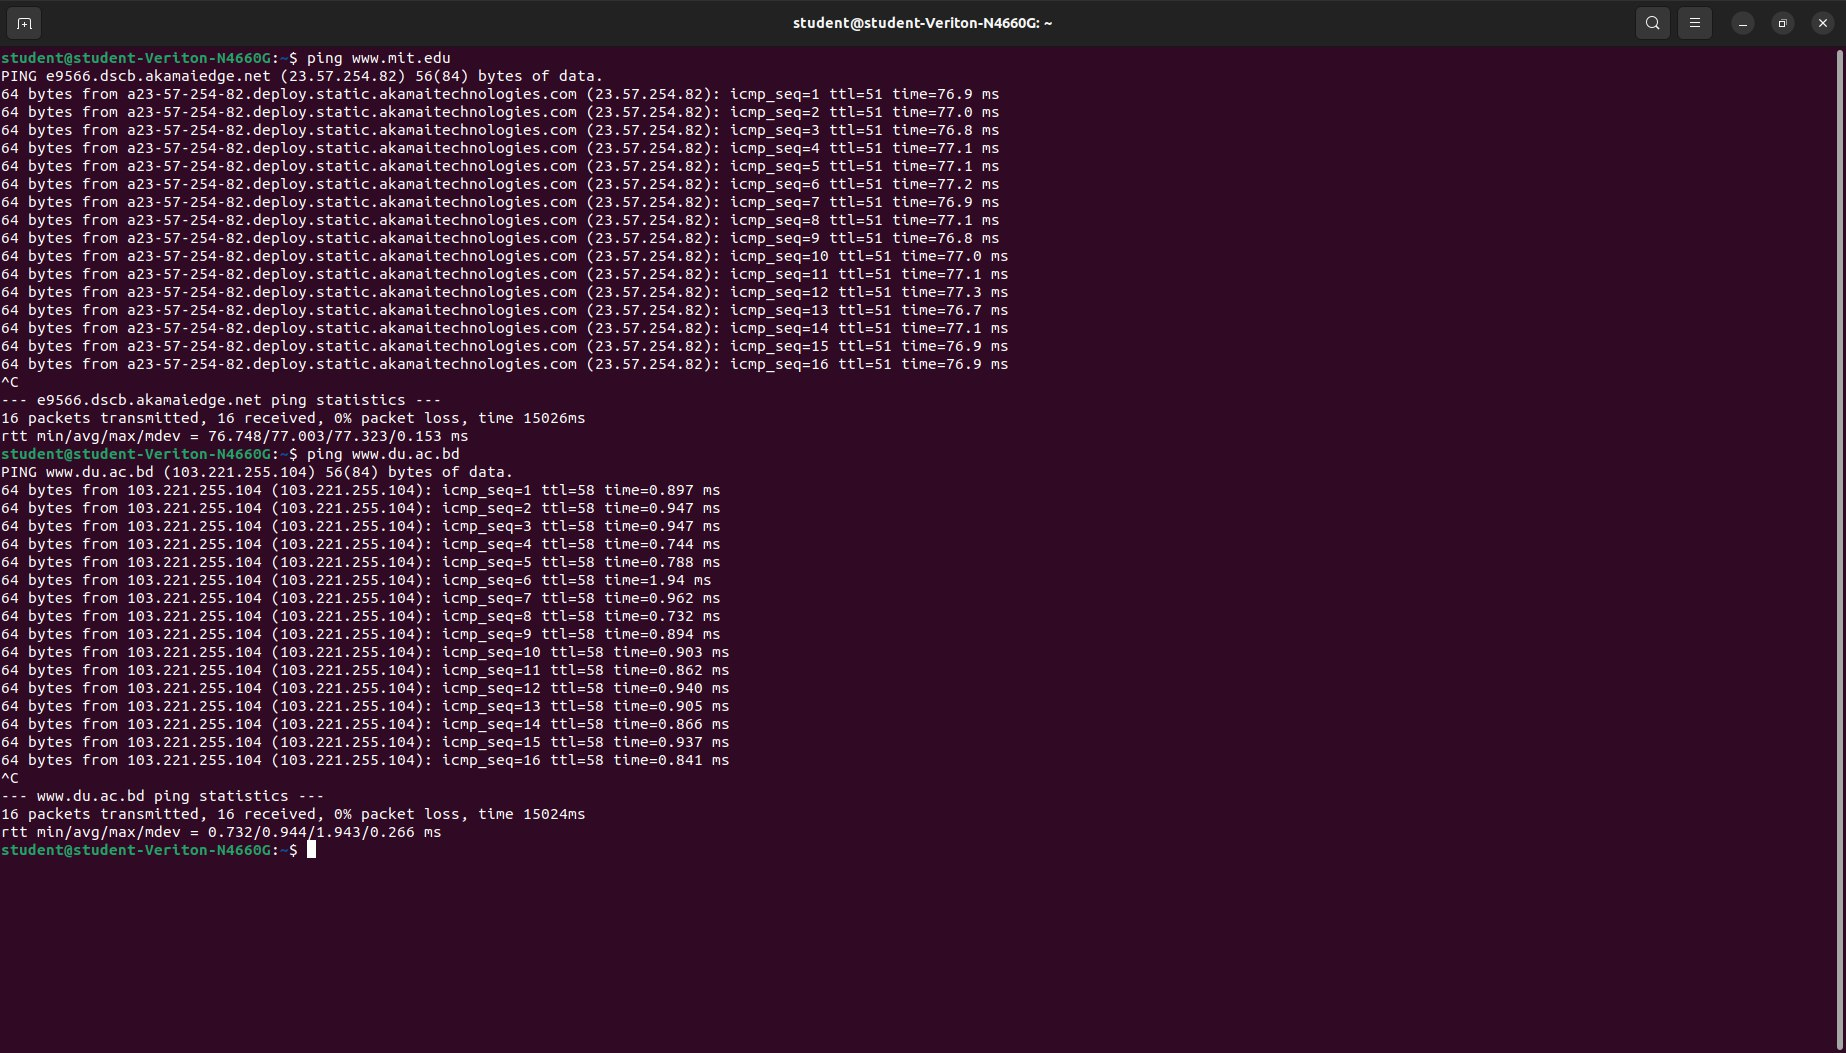
\includegraphics[width=\textwidth]{ping 1.jpg}
\caption{Result of some ping commands}
\end{figure}

\begin{figure}
\centering
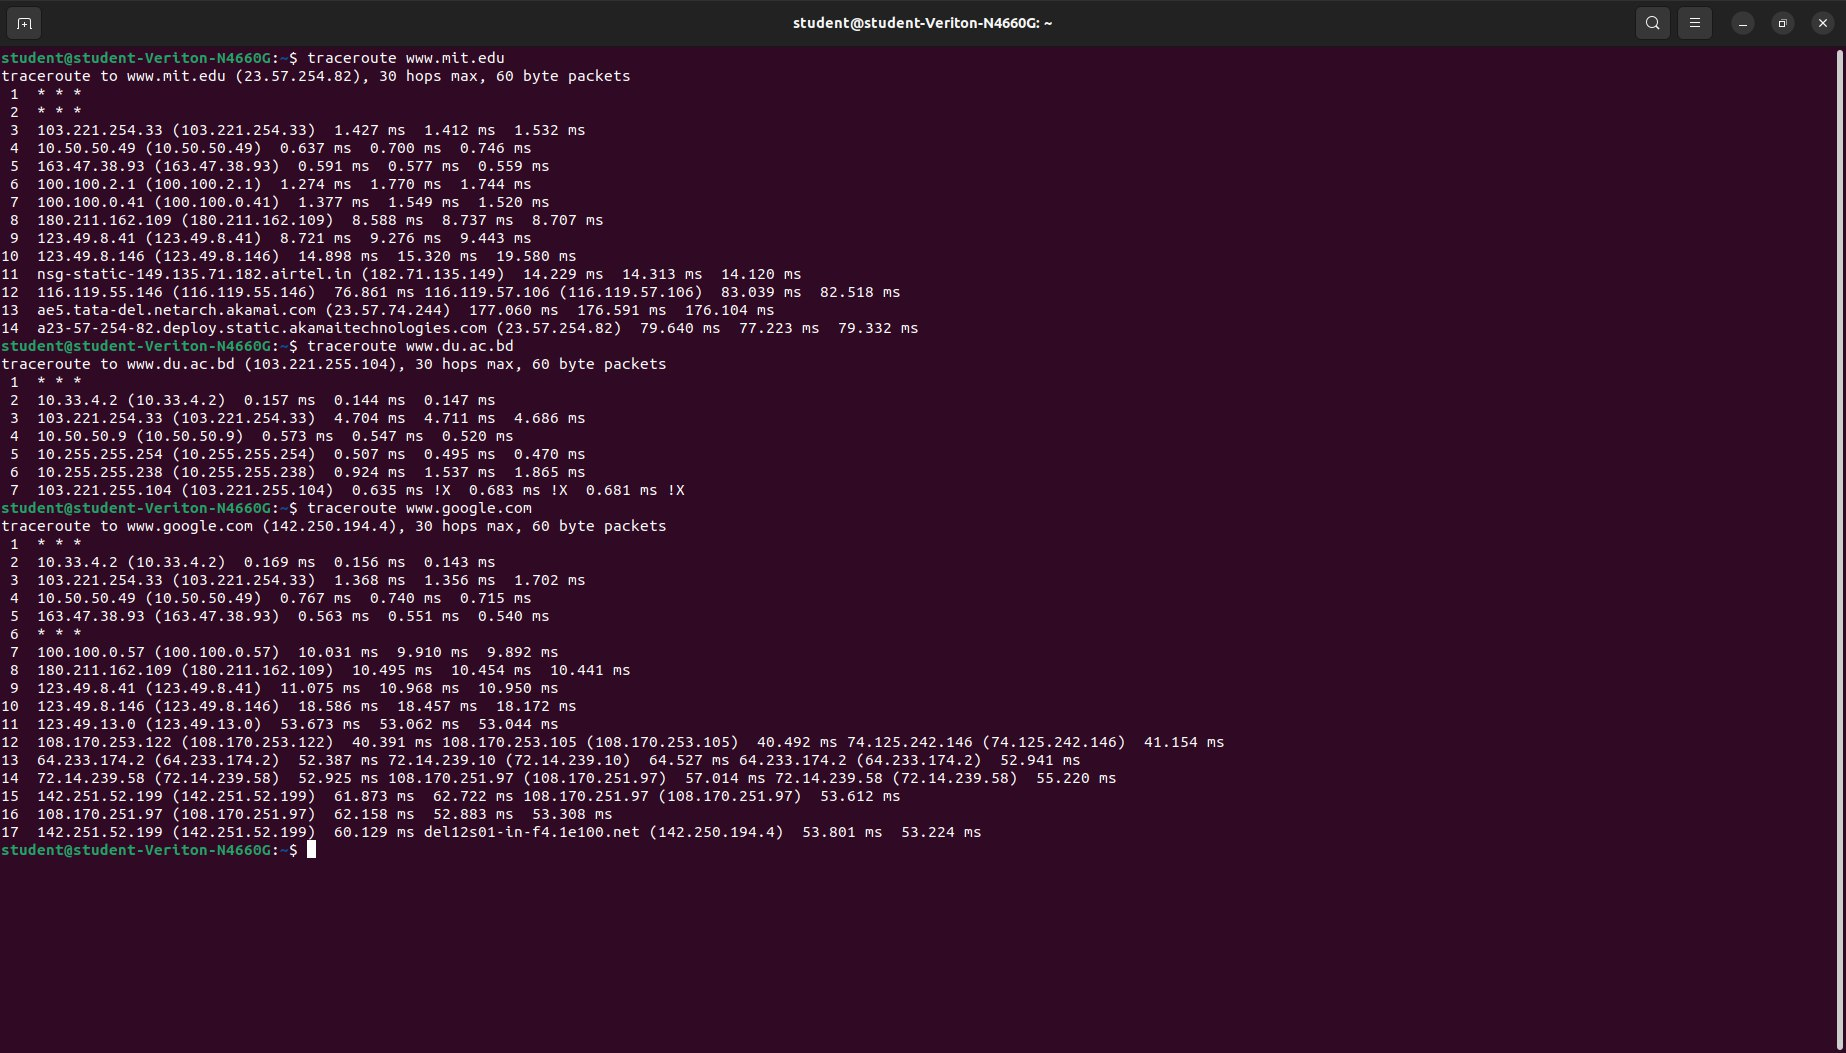
\includegraphics[width=\textwidth]{traceroute 2.jpg}
\caption{Result of some traceroute commands (1)}
\end{figure}

\begin{figure}
    \centering
    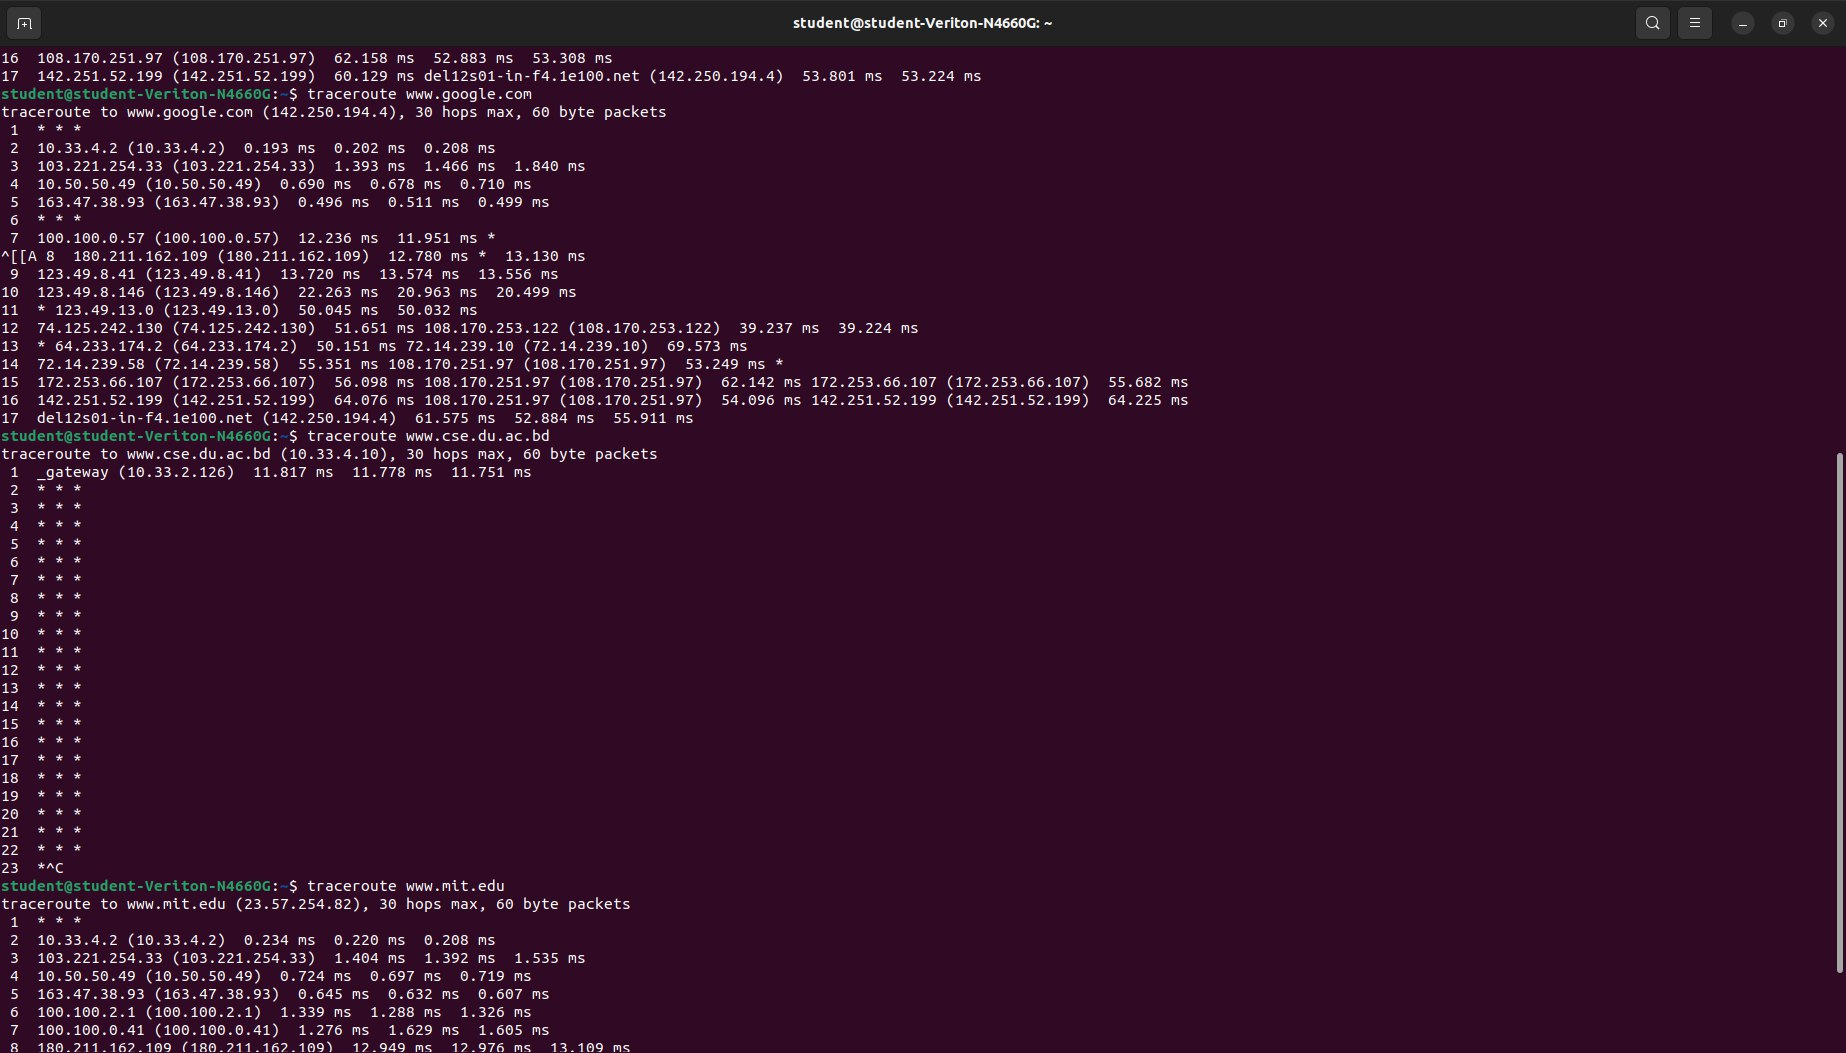
\includegraphics[width=\textwidth]{traceroute 3.jpg}
    \caption{Result of some traceroute commands (2)}
\end{figure}

\begin{figure}
    \centering
    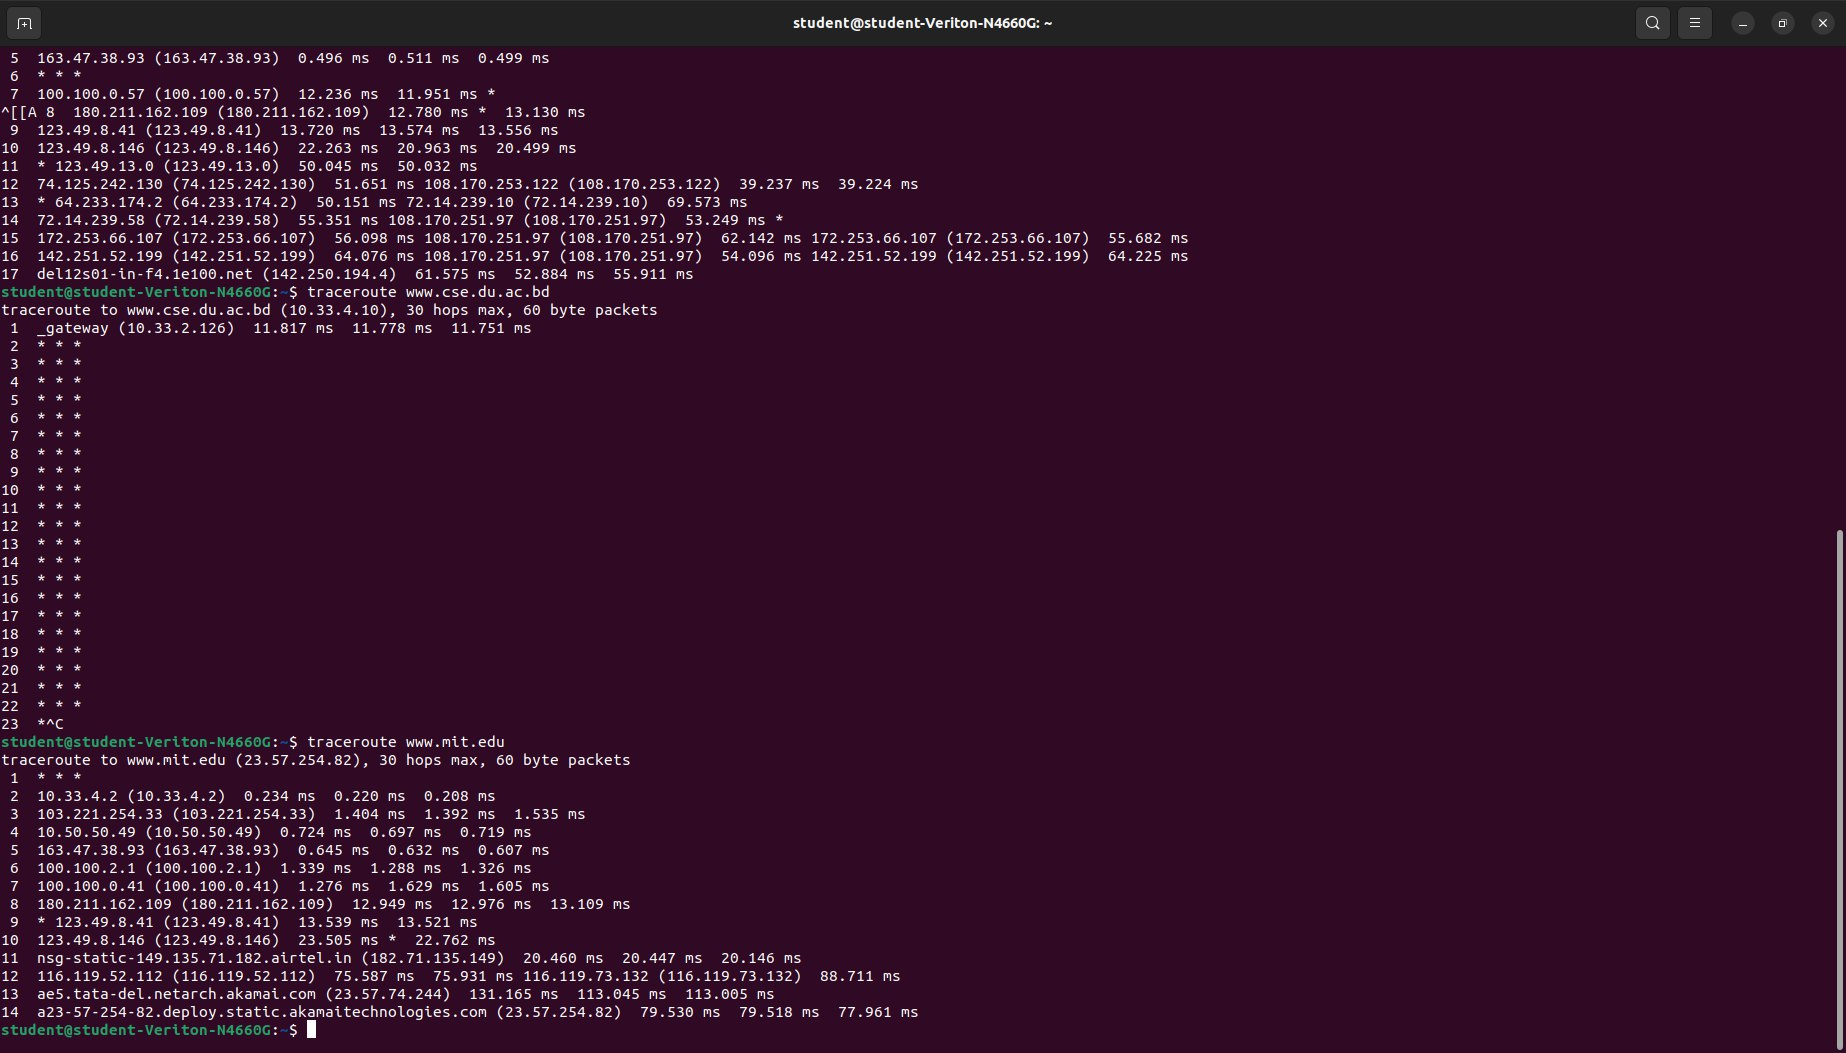
\includegraphics[width=\textwidth]{traceroute 4.jpg}
    \caption{Result of some traceroute commands (3)}  
\end{figure}

\begin{figure}
    \centering
    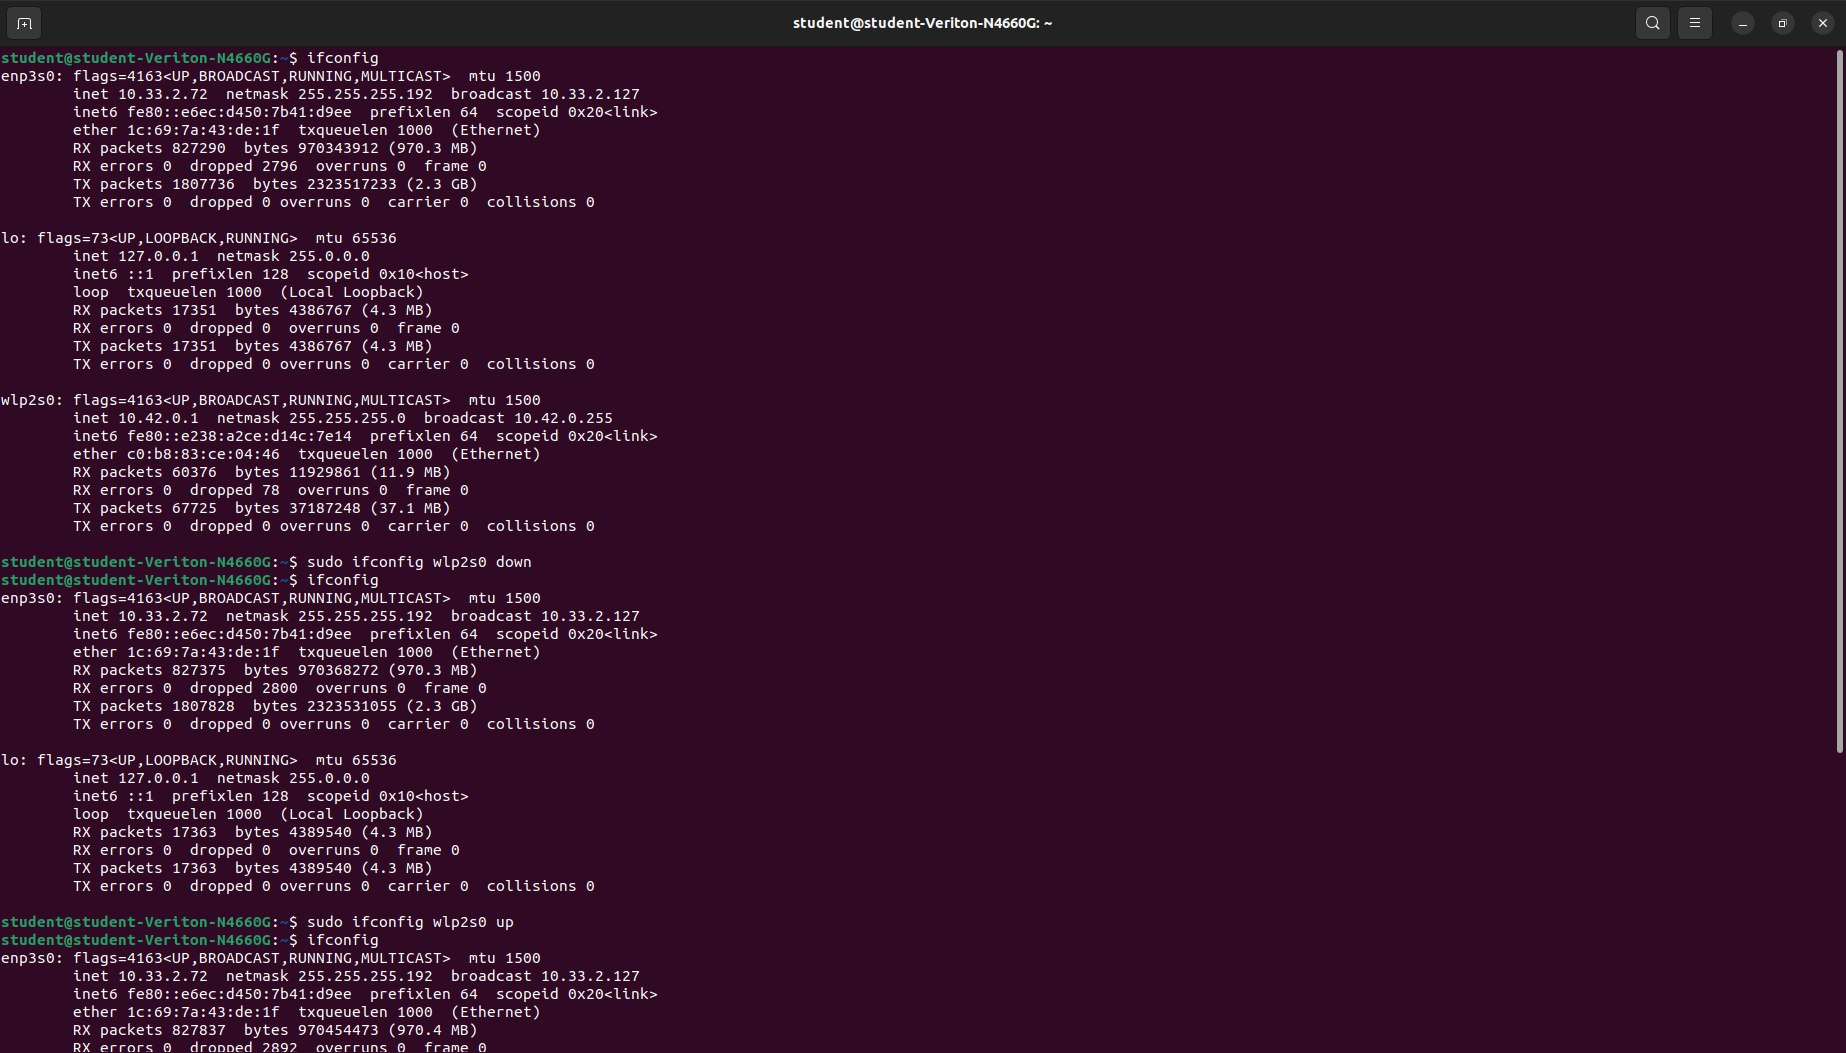
\includegraphics[width=\textwidth]{ifconfig 5.jpg}
    \caption{Result of some ifconfig commands (1)}  
\end{figure}

\begin{figure}
    \centering
    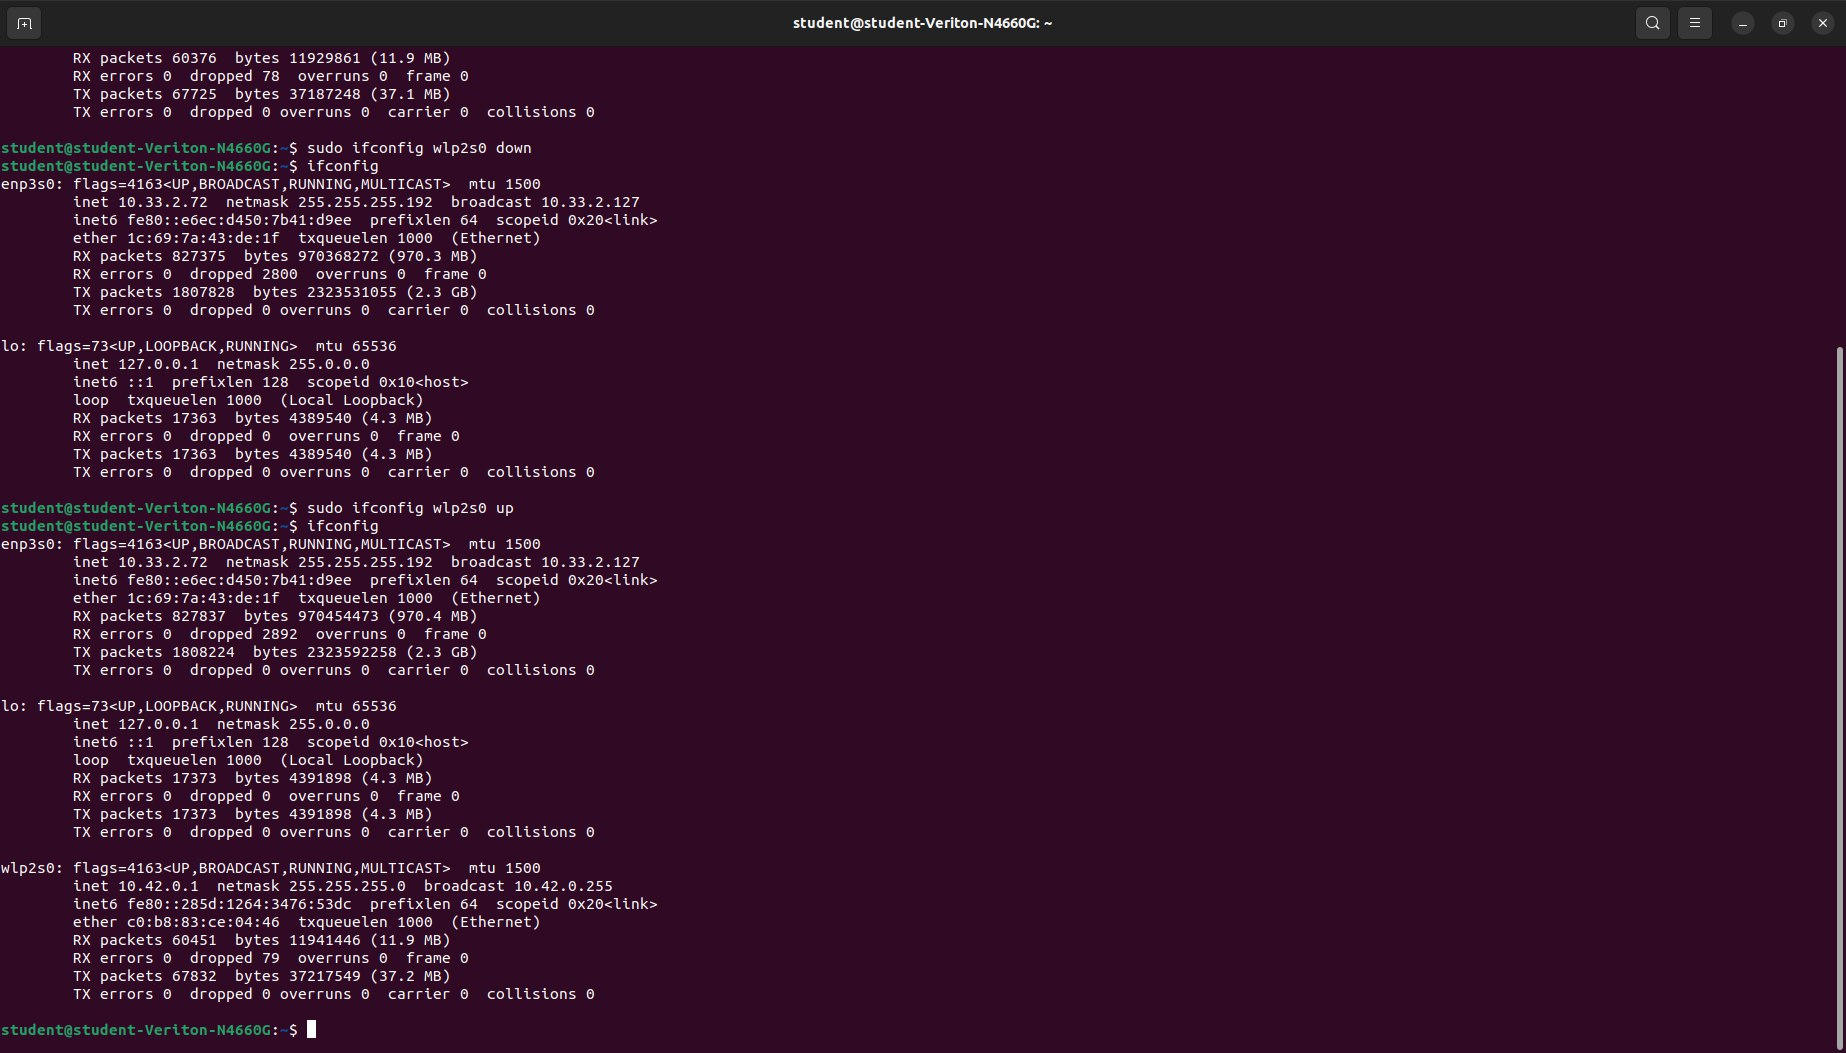
\includegraphics[width=\textwidth]{ifconfig 6.jpg}
    \caption{Result of some ifconfig commands (2)}  
\end{figure}

\begin{figure}
    \centering
    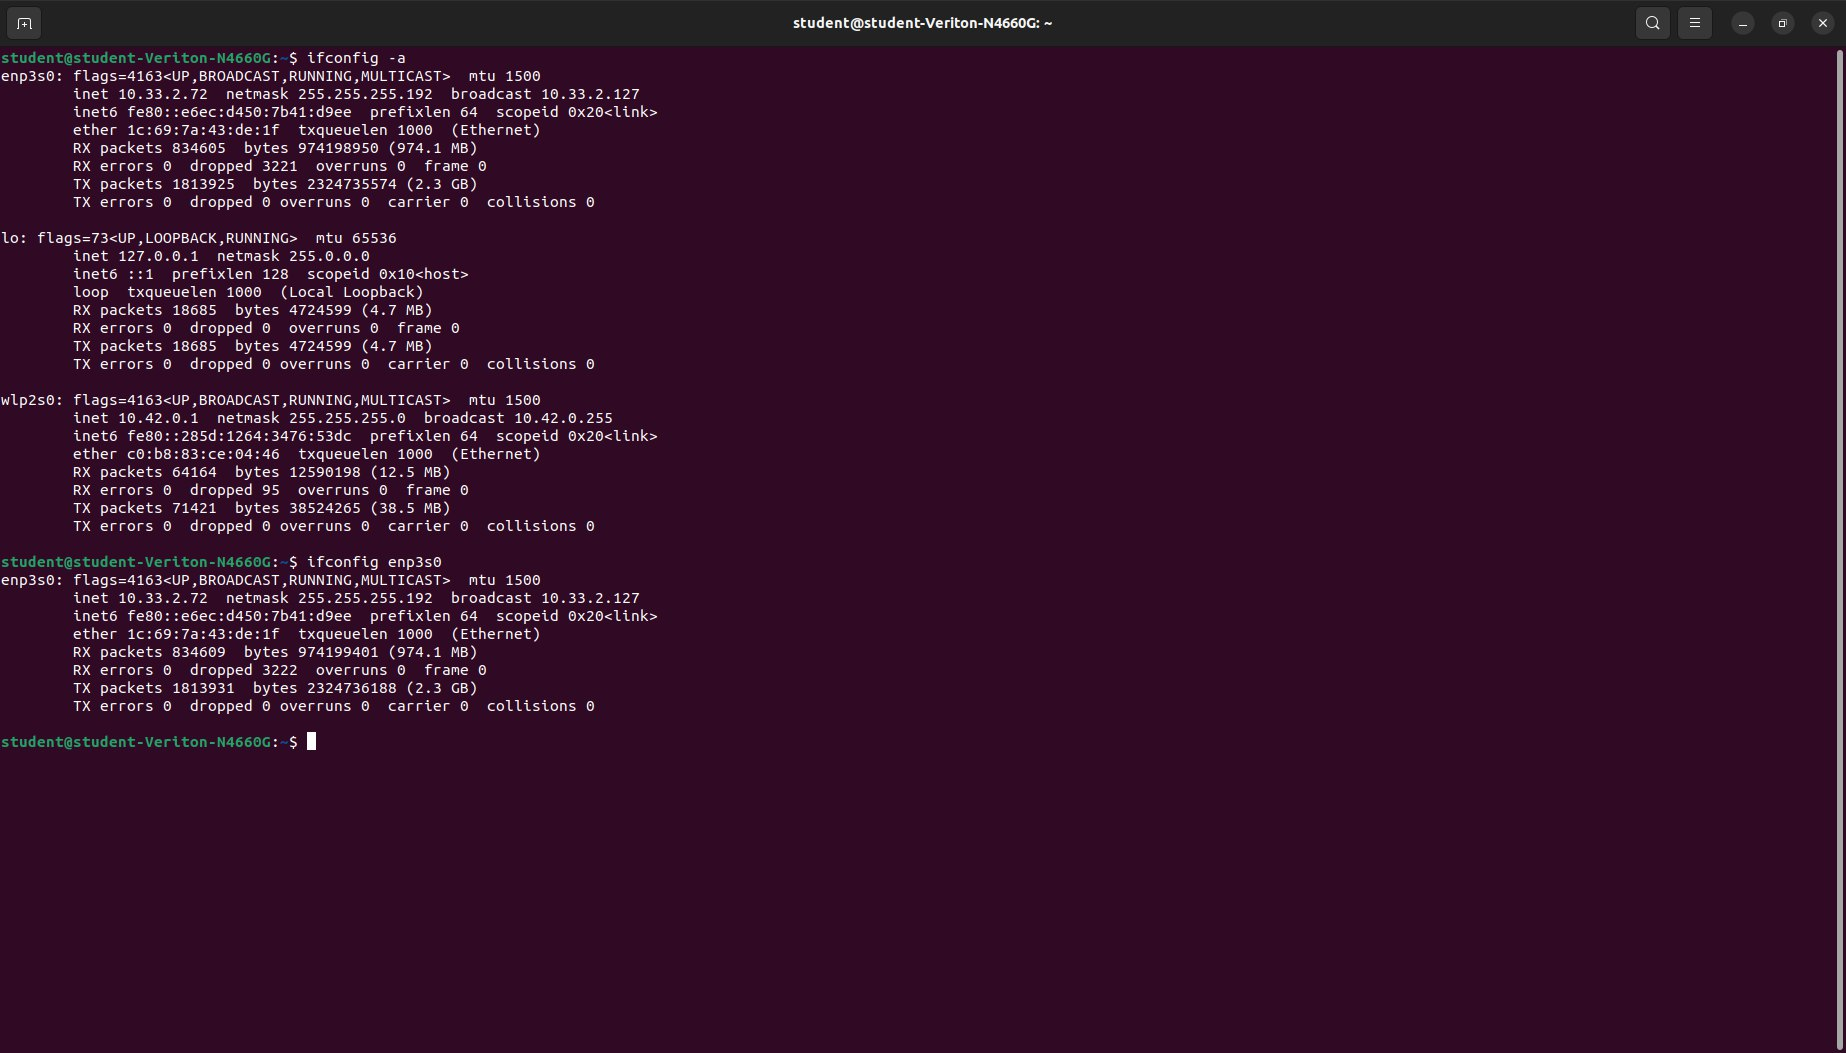
\includegraphics[width=\textwidth]{ifconfig 7.jpg}
    \caption{Result of some ifconfig commands (3)}  
\end{figure}

\begin{figure}
    \centering
    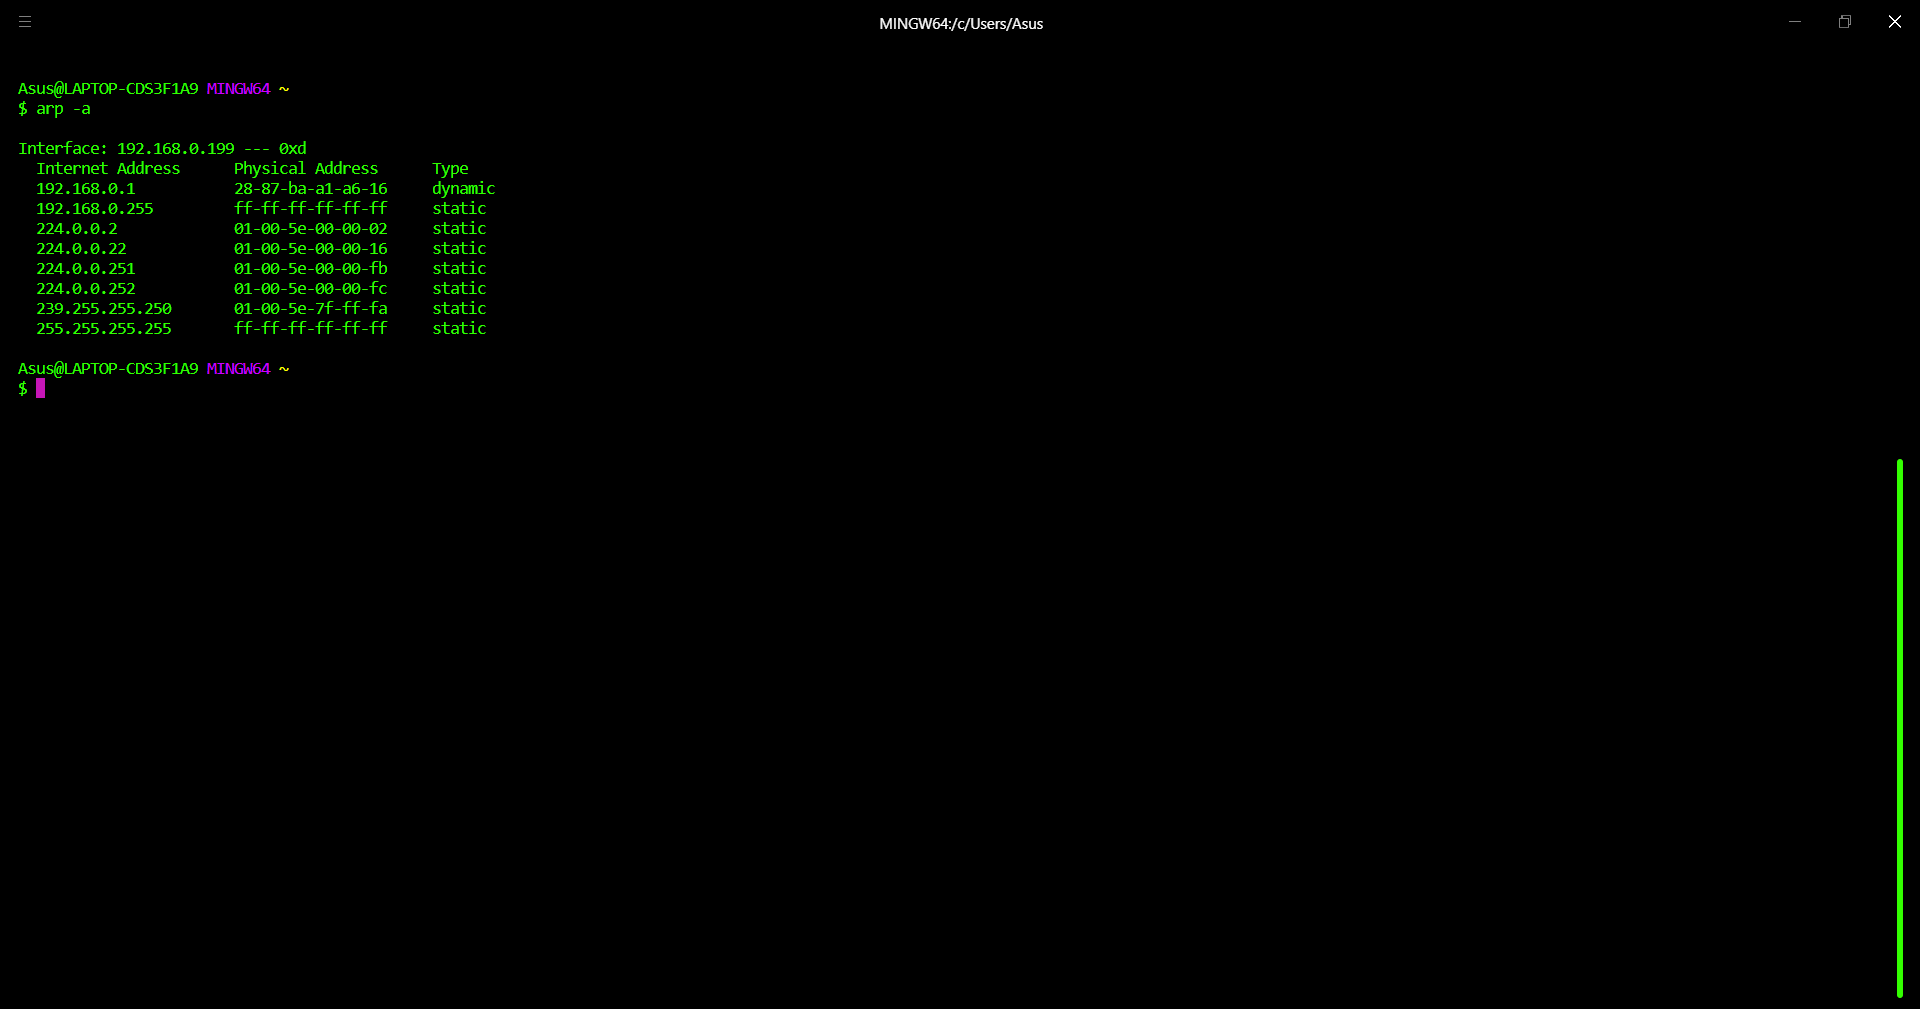
\includegraphics[width=\textwidth]{arp 1.png}
    \caption{Result of arp -a command}  
\end{figure}

\begin{figure}
    \centering
    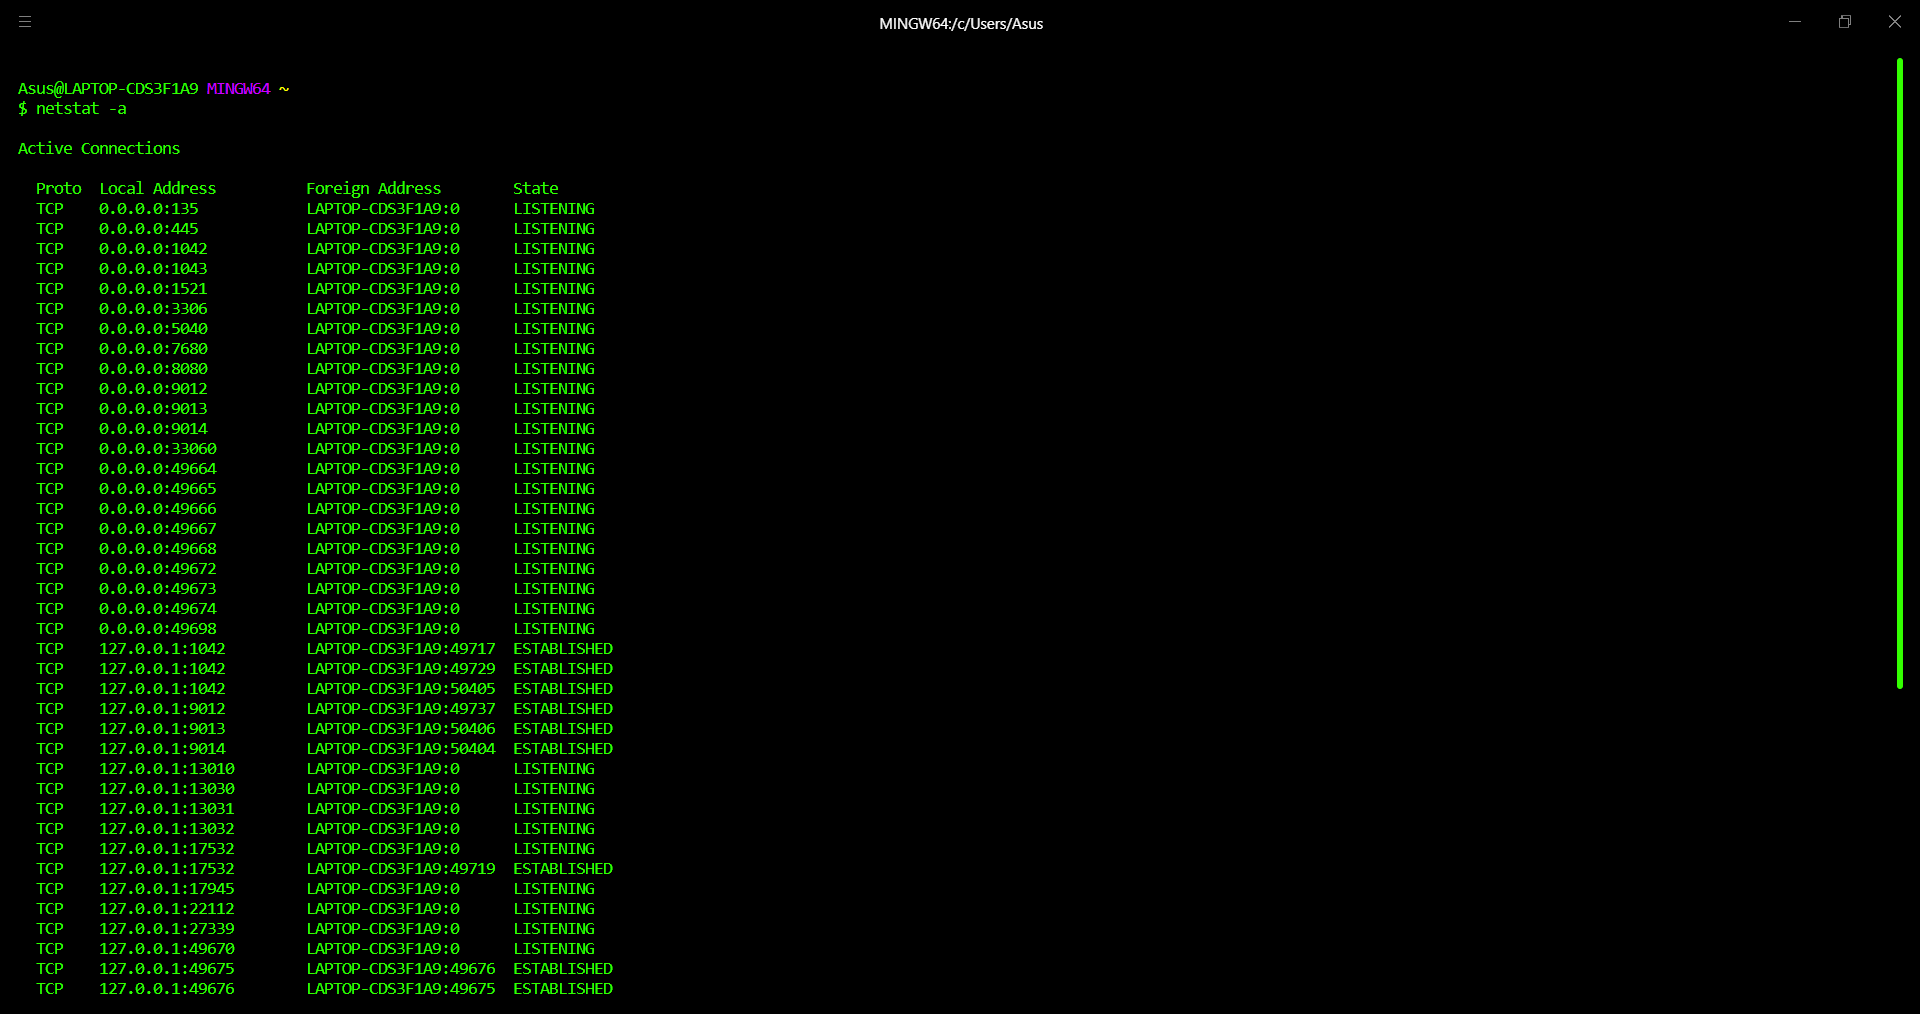
\includegraphics[width=\textwidth]{netstat 1.png}
    \caption{Result of netstat -a command}  
\end{figure}

\begin{figure}
    \centering
    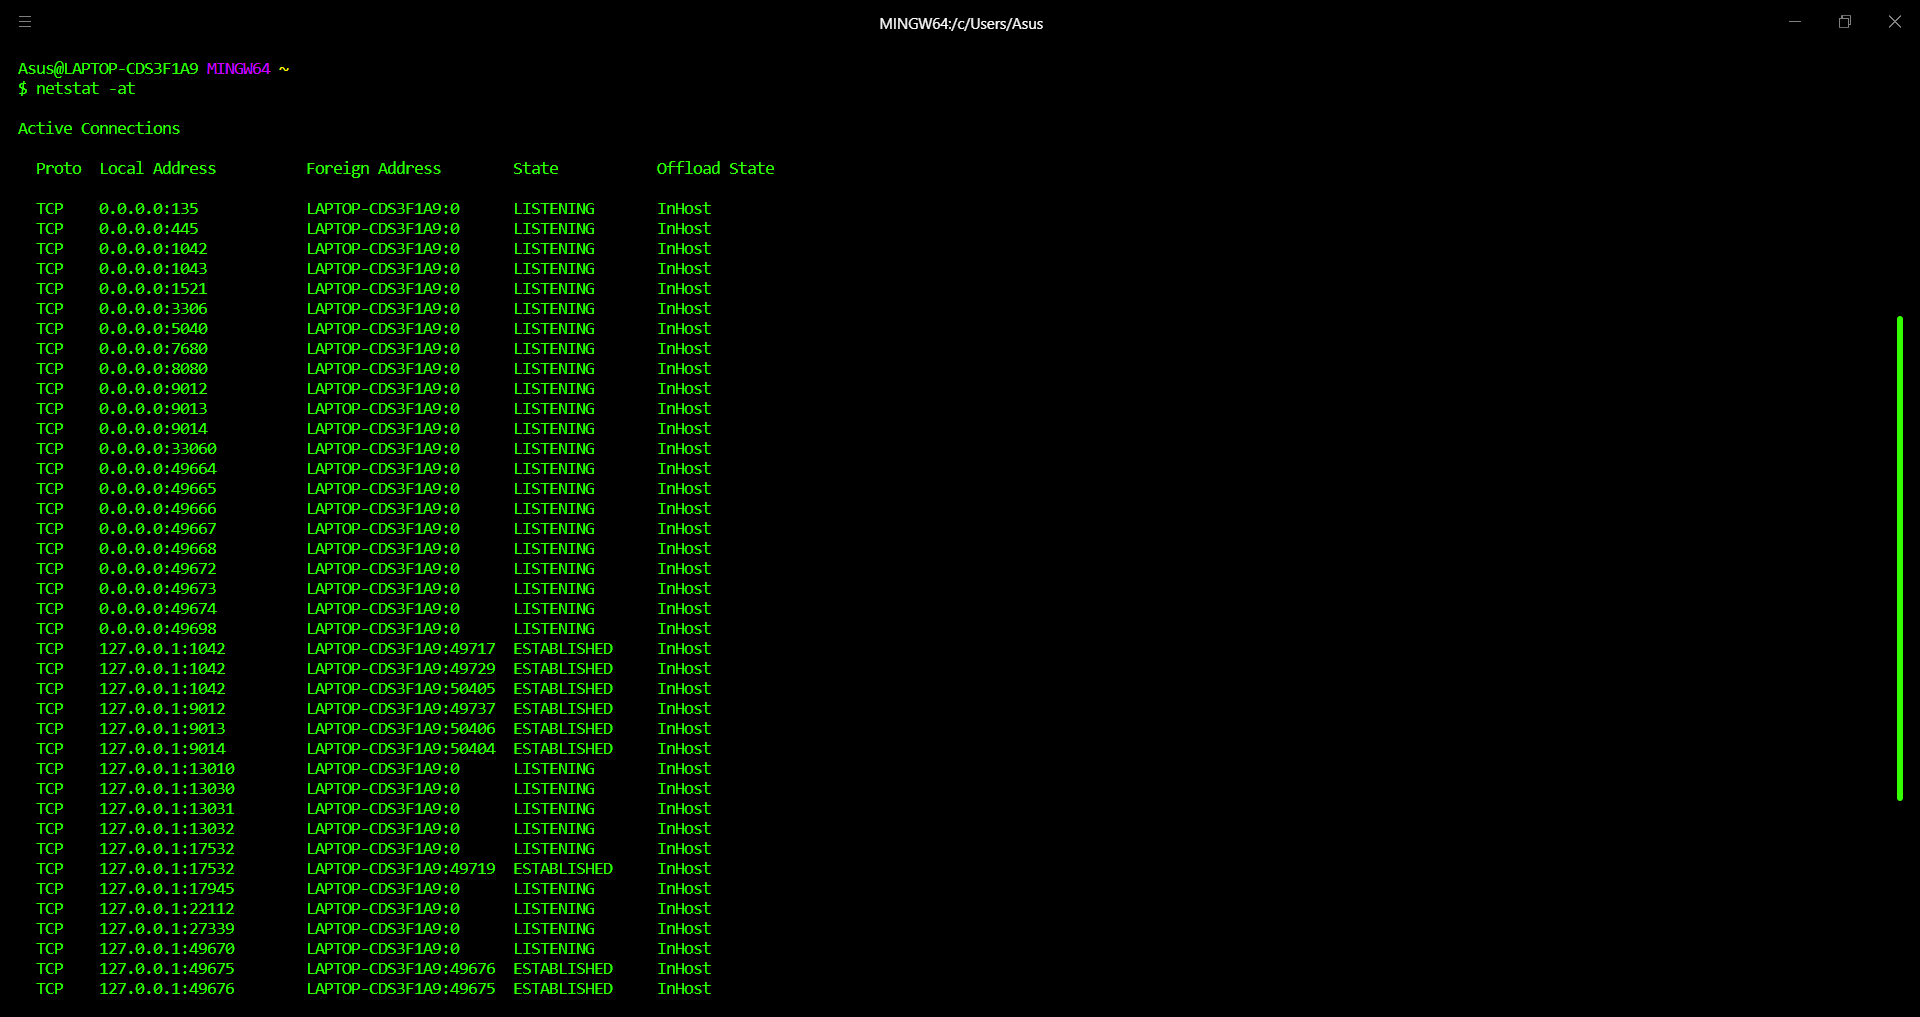
\includegraphics[width=\textwidth]{netstat 2.png}
    \caption{Result of netstat -at command}  
\end{figure}

\begin{figure}
    \centering
    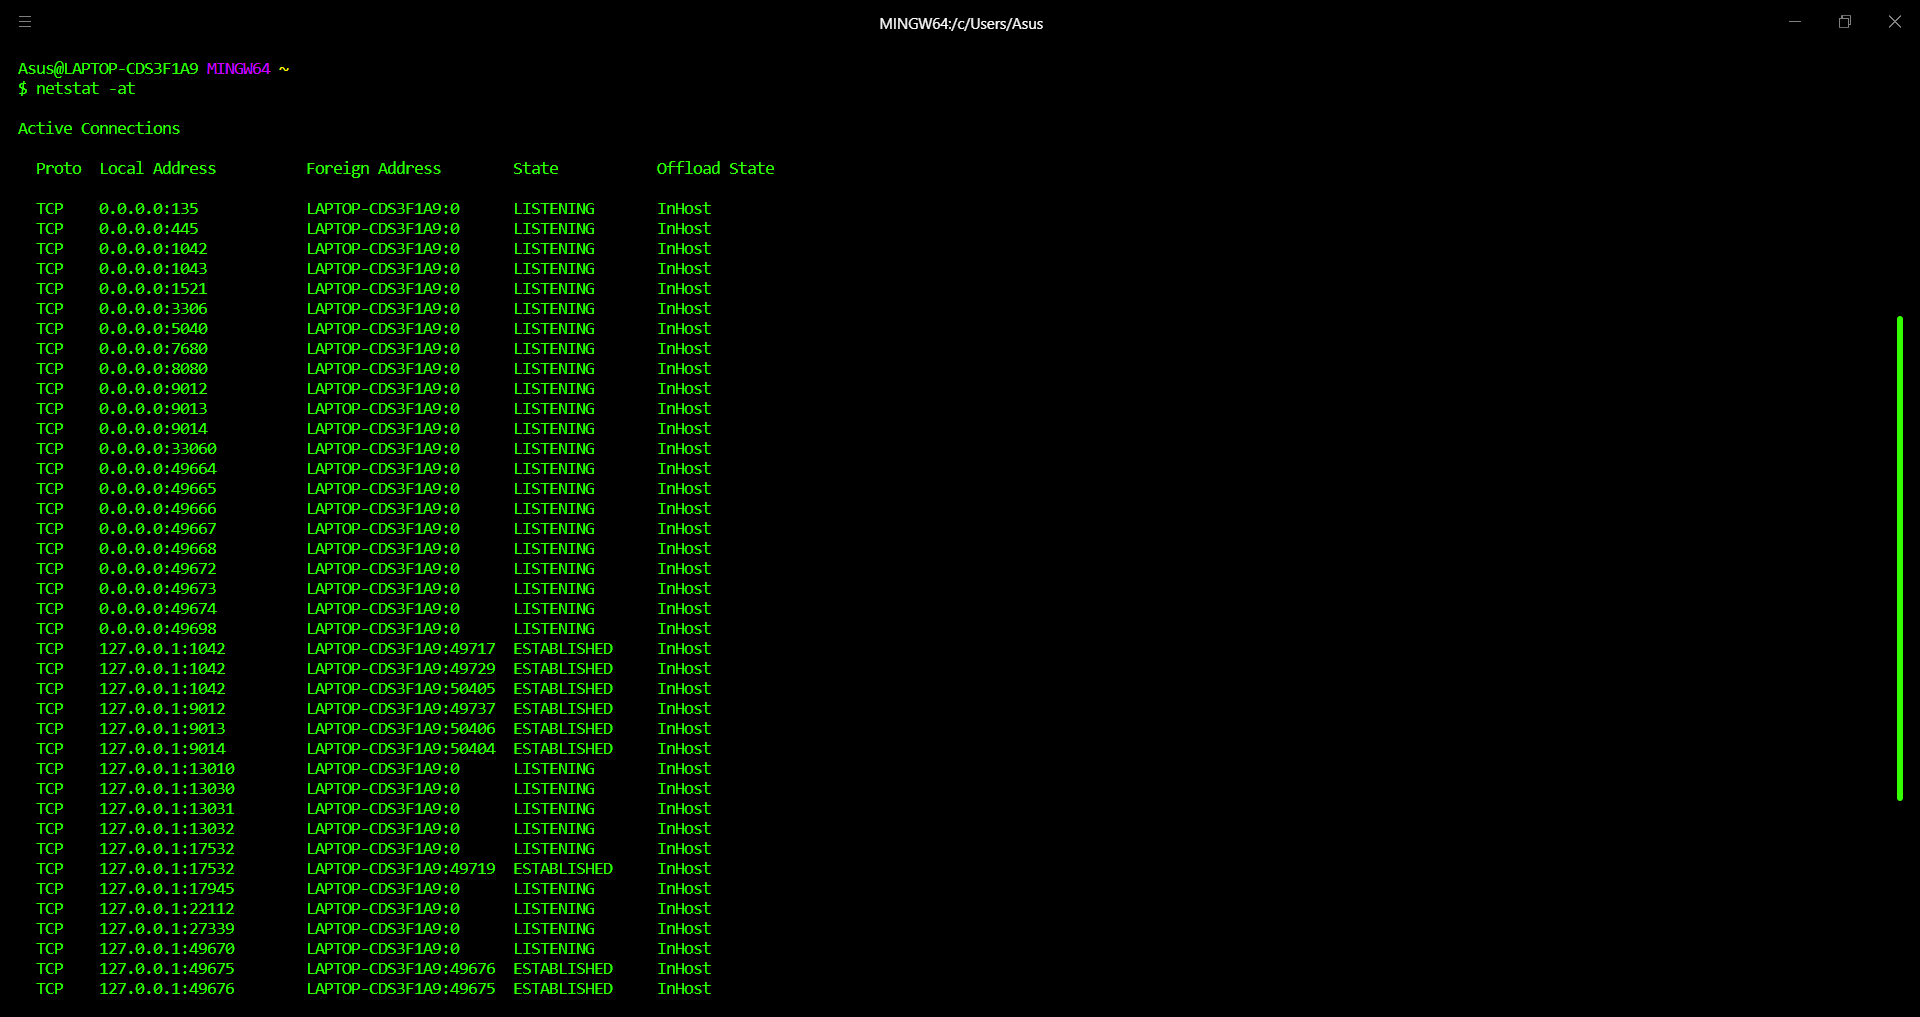
\includegraphics[width=\textwidth]{netstat 2.png}
    \caption{Result of netstat -i command}  
\end{figure}

\begin{figure}
    \centering
    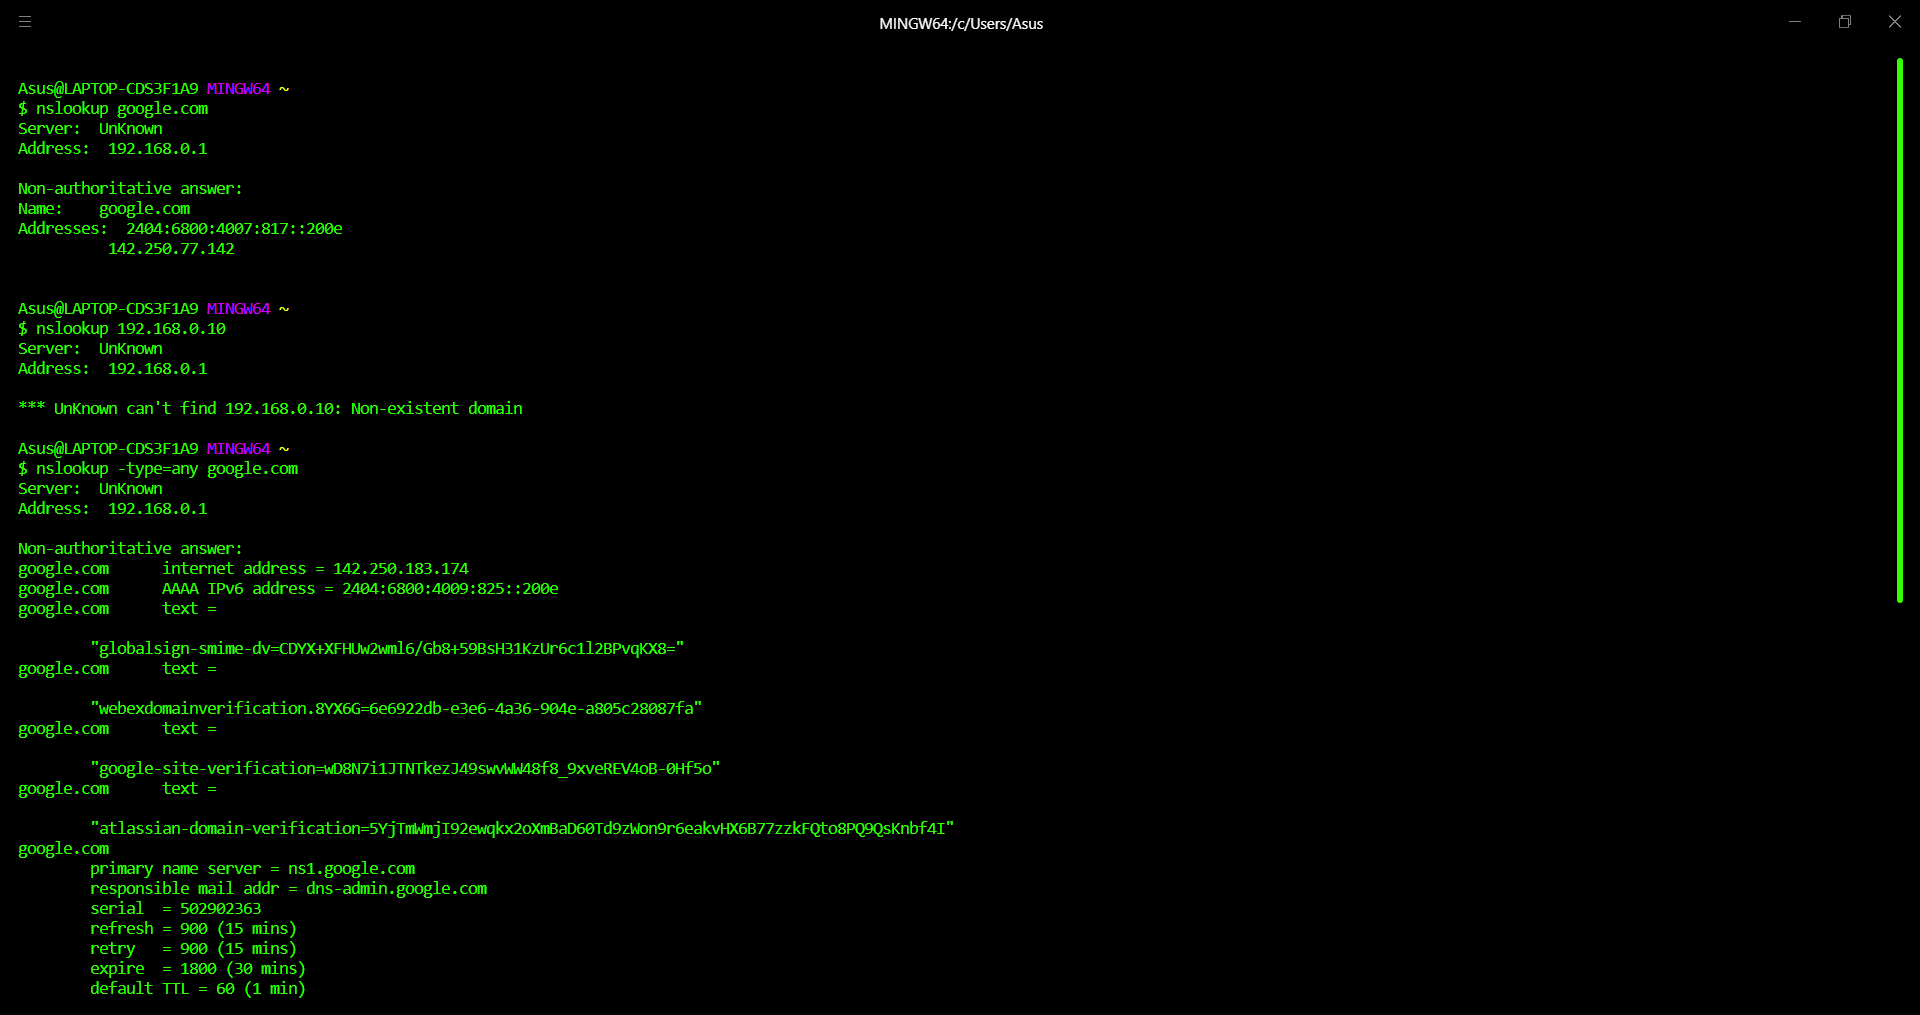
\includegraphics[width=\textwidth]{nslookup 1.png}
    \caption{Result of some nslookup commands (1)}  
\end{figure}

\begin{figure}
    \centering
    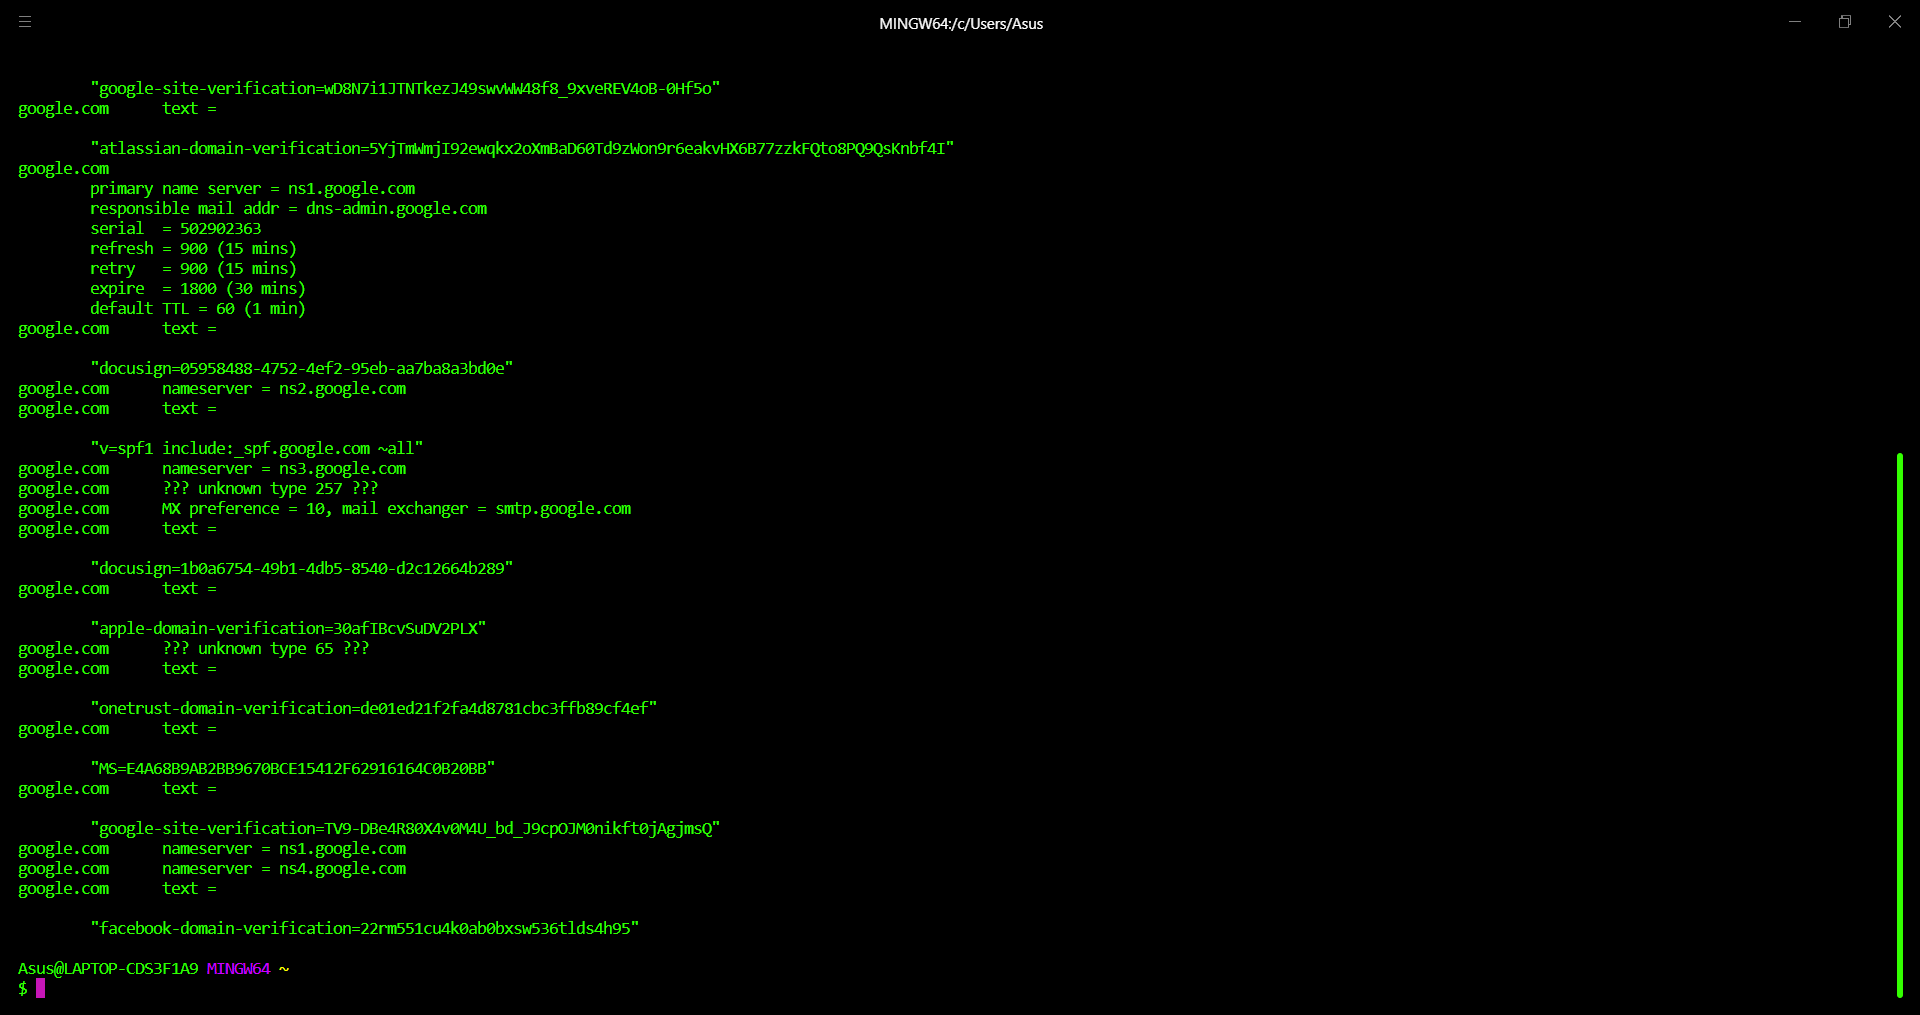
\includegraphics[width=\textwidth]{nslookup 2.png}
    \caption{Result of some nslookup commands (2)}  
\end{figure}

\newpage
\section{Experience}
\begin{enumerate}
\item Sometimes different outputs were shown for the same command in different PC's
\end{enumerate}

\begin{thebibliography}{1}
\bibitem{book}  Computer networking : a top-down approach 6th ed.
\bibitem{ChatGPT} ChatGPT : \url{https://chat.openai.com/}
\bibitem{GeeksforGeeks} GeeksforGeeks : \url{https://www.geeksforgeeks.org/}
\end{thebibliography}

\end{document}